\documentclass[aps,pre,twocolumn,showpacks,nofootinbib,superscriptaddress]{revtex4-2}

\usepackage{amsmath,amssymb}
\usepackage{graphicx}
\usepackage{bm}
\usepackage[colorlinks=true,allcolors=blue]{hyperref}

\graphicspath{{../figures/}}

\newcommand{\dd}[2]{\frac{d #1}{d #2}}
\newcommand{\phifull}{\varphi_{\mathrm{full}}}
\newcommand{\Pifull}{\Pi_{\mathrm{full}}}
\newcommand{\phiR}{\varphi_{R}}
\newcommand{\PiR}{\Pi_{R}}

\begin{document}

\title{A universal numerical renormalization method for the\\
       combined Duffing--Van der Pol oscillator}

\author{(author list)}
\affiliation{Universidad de Ingenier\'ia y Tecnolog\'ia -- UTEC,
Jr. Medrano Silva 165, Lima, Per\'u}

\date{\today}

\begin{abstract}
We present a single, \emph{universal} numerical renormalization engine, based
on the dynamical renormalization group (DRG), that constructs accurate
approximate solutions of the harmonic oscillator deformed simultaneously by a
Duffing cubic stiffness and a Van der Pol nonlinear damping. Working only with
the first-order perturbative response, the method extracts amplitude- and
phase-flow generators by projecting the secular growth of the perturbation onto
the tangent directions of the background solution. Because the first-order
problem is linear, the Duffing and Van der Pol generators superpose, so the
same engine reproduces the pure Duffing frequency shift
$\beta_\theta=\tfrac38 A^2$ (recovering the Bender--Orszag multiple-scales
result), the pure Van der Pol amplitude flow $\beta_A=\tfrac12 A(1-A^2/4)$ with
its limit cycle at $A=2$, and the combined dynamics---for arbitrary deformation
strengths and free of secular divergences. We benchmark the integrators used
for the reference solution and discuss the method's accuracy from the weak- to
the strong-coupling regime.
\end{abstract}

\maketitle

\section{Introduction}
\label{sec:intro}

Control system engineering integrates efficient process design with technical
forecasting and underpins applications in manufacturing, transportation, and
environmental management~\cite{dorf2018}. A central difficulty is selecting a
mathematical framework that captures how a system responds to internal and
external fluctuations. Differential equations provide such a framework, but
exact solutions are rarely attainable, and perturbation theory---while
powerful---often develops singular (secular) behaviour that grows without bound
in time.

One technique that tames secular growth is the dynamical renormalization group
(DRG)~\cite{chen1994,chen1996}, which reuses the first-order perturbative
solution to reparameterize the background, capturing the nonlinear features of
the dynamics as the parameters flow in time. Obtaining closed-form perturbative
solutions is not always possible, so the DRG has been adapted to accept both
analytic and numerical input~\cite{galvez2021}. In this work we build a
\emph{numerical} DRG that, from the first-order response alone, produces
solutions of the Duffing and Van der Pol equations as deformations of the simple
harmonic oscillator, and---our main contribution---of the two deformations
acting \emph{together}, through a single universal engine.

Section~\ref{sec:method} introduces the method and its numerical
implementation, reproducing the Duffing (frequency-shift) and Van der Pol
(amplitude-flow) cases. Section~\ref{sec:combined} develops the combined
Duffing--Van der Pol (DVdP) problem and shows how the independent generators
superpose. Section~\ref{sec:benchmark} benchmarks the numerical integrators and
the accuracy of the renormalized solution across coupling strengths.
Section~\ref{sec:cases} discusses case studies relevant to nonlinear control,
and Section~\ref{sec:discussion} concludes.

\section{Method of numerical renormalization}
\label{sec:method}

\subsection{Deforming the harmonic oscillator}
\label{sec:duffing}

We start from the harmonic oscillator written as a first-order system,
\begin{equation}
  \dd{\varphi^{(0)}}{t}=\Pi^{(0)}, \qquad
  \dd{\Pi^{(0)}}{t}=-\omega^2\varphi^{(0)},
  \label{eq:sho}
\end{equation}
and deform it into the damping- and force-free Duffing equation,
\begin{subequations}
\begin{align}
  \dd{\phifull}{t}&=\Pifull,\\
  \dd{\Pifull}{t}&=-\omega^2\phifull-\epsilon\,\phifull^3,
  \label{eq:duffing}
\end{align}
\end{subequations}
by a cubic correction controlled by the tunable parameter $\epsilon$. With
maximum initial amplitude set to one,
\begin{equation}
  \varphi^{(0)}(t)=\cos\varphi_\circ,\qquad
  \Pi^{(0)}(t)=-\omega\sin\varphi_\circ,
  \label{eq:background1}
\end{equation}
where $\varphi_\circ=\omega t$ is the oscillation phase, obeying
$d\varphi_\circ/dt=\omega$.

Since Eq.~\eqref{eq:duffing} is nonlinear, we seek small corrections to the
background,
\begin{equation}
  \phifull\approx\varphi^{(0)}+\epsilon\varphi^{(1)}, \qquad
  \Pifull\approx\Pi^{(0)}+\epsilon\Pi^{(1)},
  \label{eq:ansatz}
\end{equation}
Substituting into Eq.~\eqref{eq:duffing} and collecting the terms of order
$\epsilon^1$ gives the driven linear system
\begin{subequations}
\begin{align}
  \dd{\varphi^{(1)}}{t}&=\Pi^{(1)},\\
  \dd{\Pi^{(1)}}{t}&=-\omega^2\varphi^{(1)}-\bigl(\varphi^{(0)}\bigr)^3.
  \label{eq:duffing1}
\end{align}
\end{subequations}
The source $(\varphi^{(0)})^3$ acts as a resonant forcing; integrating with
$\varphi^{(1)}=\Pi^{(1)}=0$ produces an amplitude that grows after a few
oscillations. This \emph{secular growth} (Fig.~\ref{fig:secular}) is a
well-known artifact of the perturbative decomposition~\cite{bender1999,
kevorkian1981}, not of the full solution.

\begin{figure}[t]
  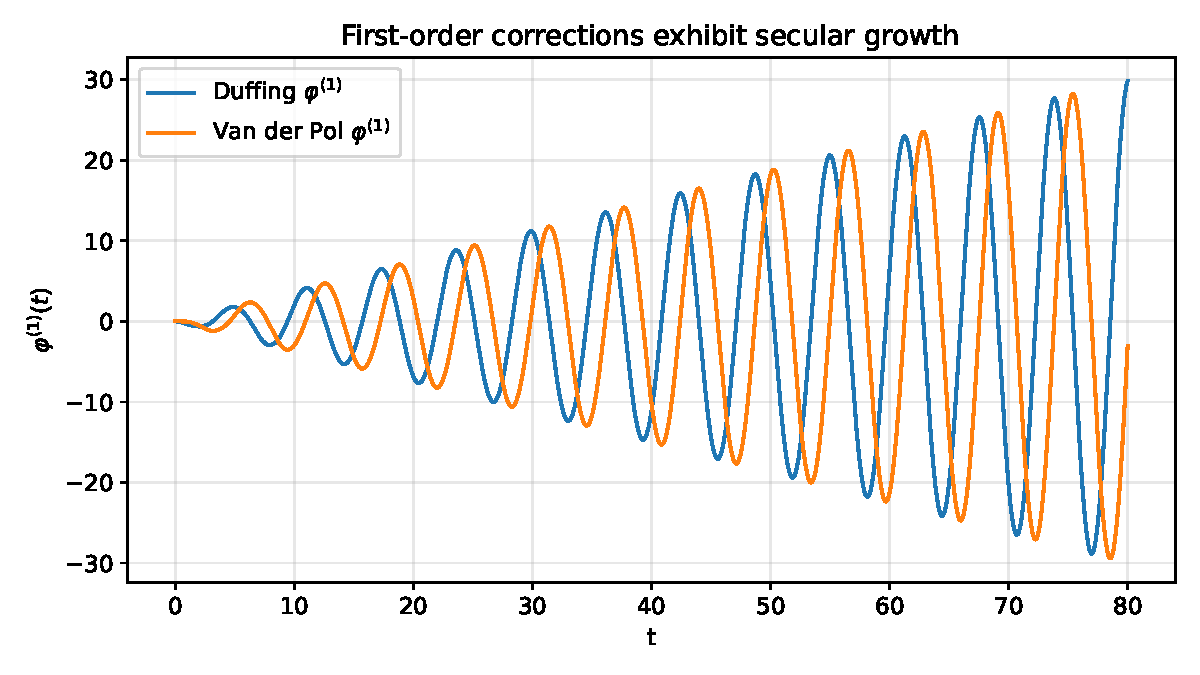
\includegraphics[width=\columnwidth]{fig_secular_growth.pdf}
  \caption{First-order corrections $\varphi^{(1)}$ for the Duffing and Van der
  Pol deformations about $A=1$. Both grow without bound in time, so the naive
  sum $\varphi^{(0)}+\epsilon\varphi^{(1)}$ fails at long times.}
  \label{fig:secular}
\end{figure}

\subsection{Renormalized solutions from first-order perturbation theory}
\label{sec:renorm}

The full Duffing solution differs from the cosine mainly in its oscillation
phase, suggesting that a time-dependent correction to the frequency and phase
suffices. We promote the background parameters
$\vec\lambda_0=(\varphi_\circ;\omega)$ to flow in time through the infinitesimal
transformation
\begin{equation}
  \vec\lambda_0(t)\to\vec\lambda_R(t)=\vec\lambda_0(t)+\epsilon\,\Delta\vec\lambda,
  \label{eq:lambdaflow}
\end{equation}
which induces the parameter-flow equations
\begin{equation}
  \dd{\varphi_\circ^R}{t}=\omega_R+\epsilon\,\alpha_\omega^{(1)}, \qquad
  \dd{\omega_R}{t}=\epsilon\,\beta_\omega^{(1)}.
  \label{eq:paramflow}
\end{equation}
The renormalized solution is obtained by inserting the flowing parameters back
into the background,
\begin{equation}
  \phifull\approx\phiR(t)\equiv\varphi^{(0)}(t,\vec\lambda_R),\qquad
  \Pifull\approx\PiR(t).
  \label{eq:renormsol}
\end{equation}

The generators are fixed by matching the first-order expansion to the expanded
renormalized solution. Writing
$\phiR=\varphi^{(0)}+\epsilon\,\nabla_{\vec\lambda_0}\varphi^{(0)}\!\cdot\Delta\vec\lambda$
and collecting the $O(\epsilon)$ terms yields the residual
\begin{equation}
  \varphi^{(1)}_{\perp,A}=\varphi^{(1)}_A-\varphi_{\parallel,A},\qquad
  \varphi_{\parallel,A}\equiv\nabla_{\vec\lambda_0}\varphi^{(0)}_A\!\cdot\Delta\vec\lambda .
  \label{eq:residual}
\end{equation}
Minimizing the cost function
\begin{equation}
  I=\sum_{A=1}^{2}\int_{t_0}^{\infty}\bigl|\varphi^{(1)}_{\perp,A}\bigr|^2\,dt
  \label{eq:cost}
\end{equation}
interprets the generators as the projection coefficients of the perturbation
$\varphi^{(1)}_A$ onto the basis of background derivatives
$\nabla_{\vec\lambda}\varphi^{(0)}_A$ (Fig.~\ref{fig:generators}). Because the
cost is quadratic, the minimization reduces to a small linear system.

\paragraph{Numerical generator extraction.} In practice we parameterize the
background by an amplitude $A$ and a phase $\theta$,
$\varphi^{(0)}=A\cos(\omega t+\theta)$, and decompose the numerically integrated
perturbation $(\varphi^{(1)},\Pi^{(1)})$ \emph{pointwise} onto the tangent
directions $\partial_A\varphi^{(0)}$ and $\partial_\theta\varphi^{(0)}$ (and
their momentum partners). A resonant generator makes the resulting coefficient
time series grow linearly; its slope is the generator. This isolates the
secular content from bounded oscillatory contributions and is numerically
robust up to strong coupling. For the Duffing oscillator we find that the
amplitude generator vanishes, $\beta_A\approx0$, while the phase generator is
\begin{equation}
  \beta_\theta^{\mathrm{Duf}}(A)=\tfrac{3}{8}A^2,
  \label{eq:betaduffing}
\end{equation}
in exact agreement with the multiple-scales result of Bender and
Orszag~\cite{bender1999} at $A=1$, $\omega=1$. Solving the flow
$d\theta/dt=\epsilon\,\beta_\theta(A)$ and reconstructing $\phiR$ gives a solution
that stays in phase with the full Duffing solution for tens of oscillations and
never diverges in amplitude (Fig.~\ref{fig:duffing}).

\begin{figure}[t]
  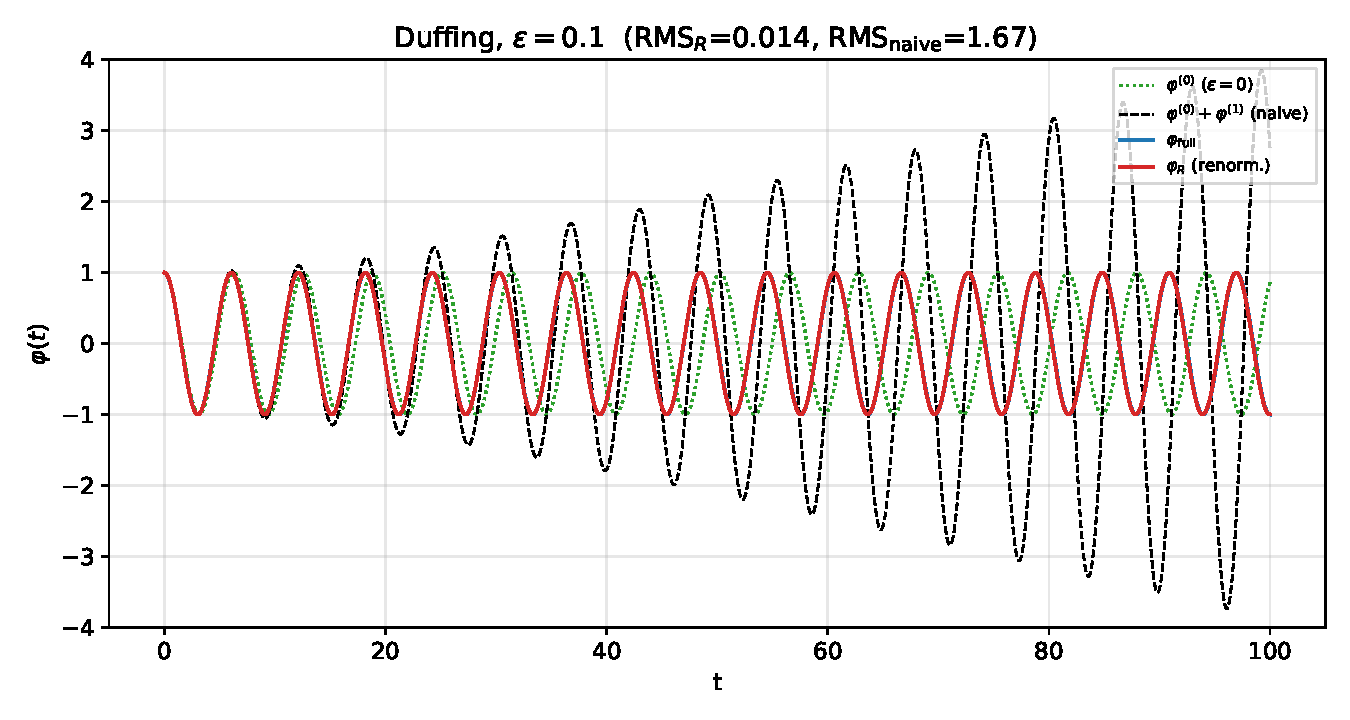
\includegraphics[width=\columnwidth]{fig_duffing_compare.pdf}
  \caption{Duffing oscillator at $\epsilon=0.1$: the full solution
  $\phifull$ (blue), the renormalized solution $\phiR$ (red) and the naive
  first-order solution $\varphi^{(0)}+\epsilon\varphi^{(1)}$ (dashed). The
  renormalized solution captures the phase evolution without secular amplitude
  growth. The RMS errors versus the full solution are quoted in the title.}
  \label{fig:duffing}
\end{figure}

\subsection{The Van der Pol oscillator}
\label{sec:vdp}

The Van der Pol oscillator is a different deformation of the harmonic
oscillator,
\begin{equation}
  \dd{\varphi}{t}=\Pi,\qquad
  \dd{\Pi}{t}=-\omega^2\varphi+\alpha\,(1-\varphi^2)\,\Pi,
  \label{eq:vdp}
\end{equation}
with strength $\alpha$. (We use the standard sign $1-\varphi^2$ of the nonlinear
damping.) Here the full solution spirals toward a limit cycle, so rather than a
frequency shift the background must be parameterized by a \emph{varying
amplitude}, $\varphi^{(0)}=A_0\cos(\omega t)$,
$\Pi^{(0)}=-\omega A_0\sin(\omega t)$. The first-order perturbation
\begin{equation}
  \dd{\Pi^{(1)}}{t}=-\omega^2\varphi^{(1)}+\Pi^{(0)}\bigl(1-(\varphi^{(0)})^2\bigr)
\end{equation}
again grows secularly; projecting it onto the amplitude direction gives the
amplitude flow
\begin{equation}
  \dd{A_R}{t}=\alpha\,\beta_A(A_R),\qquad
  \beta_A^{\mathrm{VdP}}(A)=\tfrac12 A\bigl(1-\tfrac{A^2}{4}\bigr),
  \label{eq:betavdp}
\end{equation}
whose stable zero at $A=2$ is the limit-cycle radius. The reconstructed solution
tracks the amplitude growth of the full Van der Pol solution and converges to
the correct limit cycle without secular growth (Fig.~\ref{fig:vdp}).

\begin{figure}[t]
  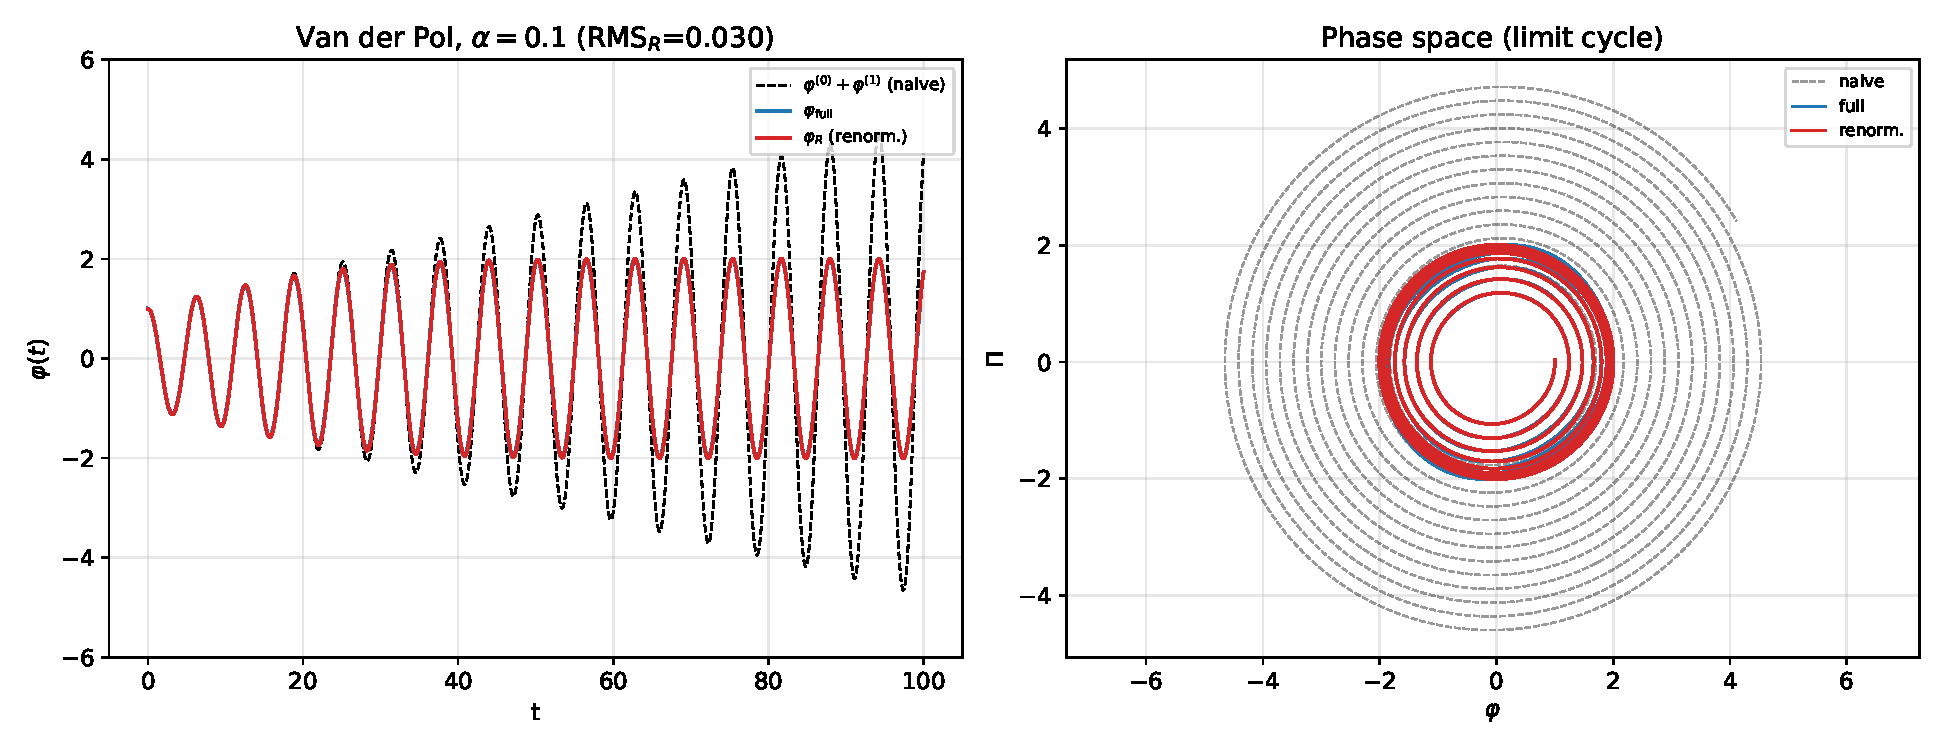
\includegraphics[width=\columnwidth]{fig_vdp_compare.pdf}
  \caption{Van der Pol oscillator at $\alpha=0.1$. Left: time series of the
  full, renormalized and naive solutions. Right: phase-space portrait; the
  renormalized amplitude flow reproduces the approach to the limit cycle.}
  \label{fig:vdp}
\end{figure}

\begin{figure}[t]
  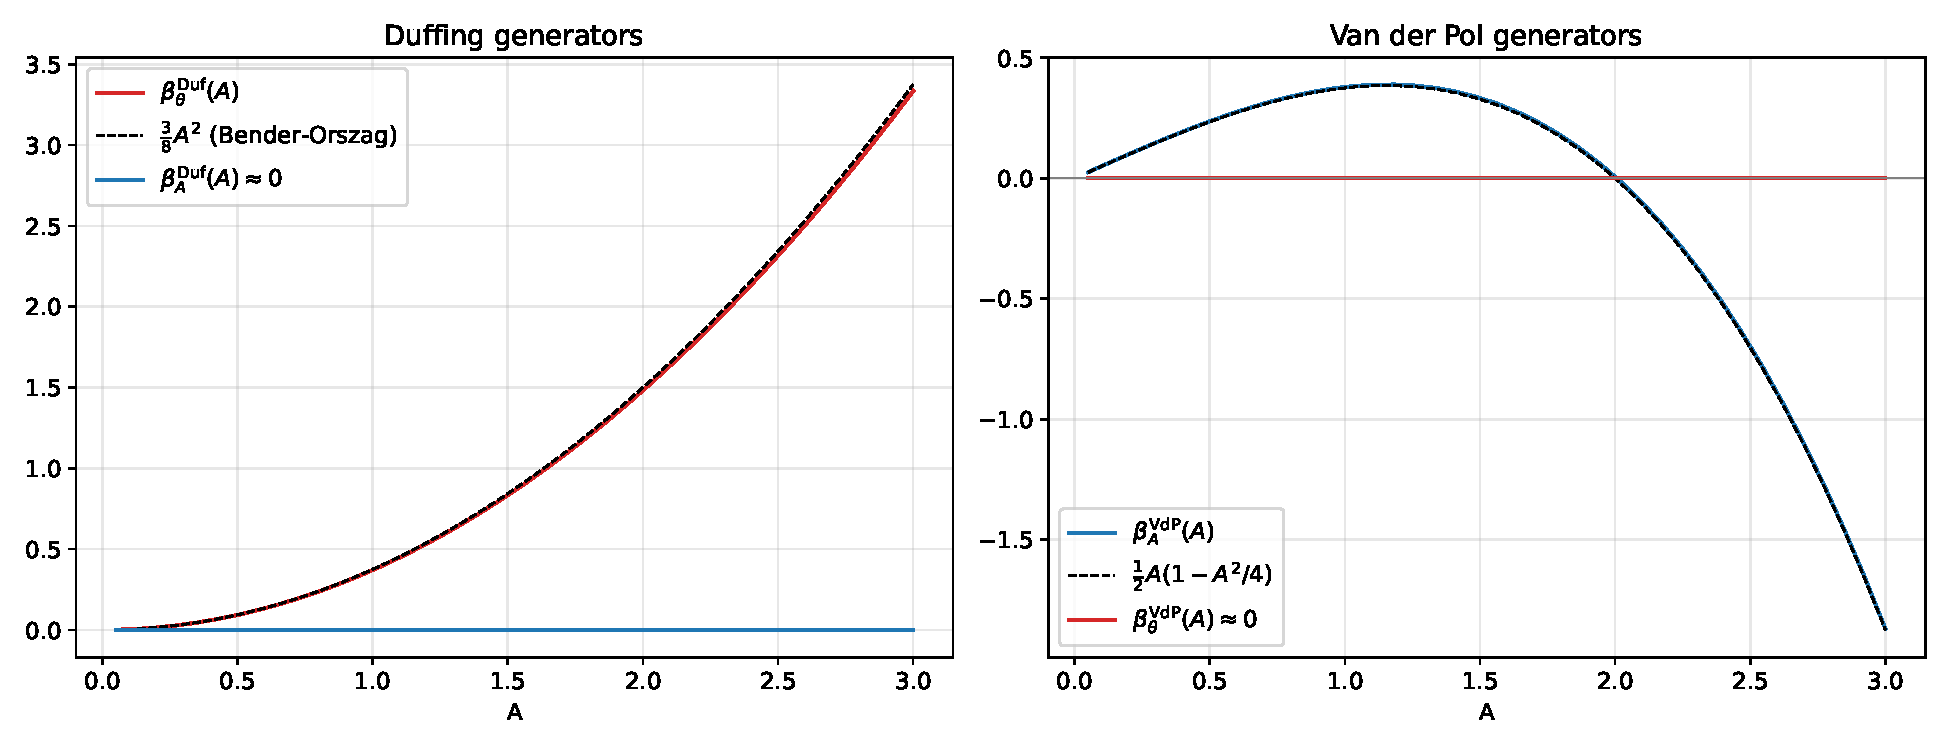
\includegraphics[width=\columnwidth]{fig_generators.pdf}
  \caption{Numerically extracted generators. Left: Duffing, where the phase
  generator follows $\tfrac38 A^2$ and the amplitude generator is consistent
  with zero. Right: Van der Pol, where the amplitude generator follows
  $\tfrac12 A(1-A^2/4)$ (zero at the limit cycle $A=2$) and the phase generator
  vanishes.}
  \label{fig:generators}
\end{figure}

\section{The combined Duffing--Van der Pol oscillator}
\label{sec:combined}

We now switch on both deformations simultaneously, with \emph{independent}
strengths $\epsilon$ (Duffing) and $\alpha$ (Van der Pol):
\begin{equation}
  \dd{\varphi}{t}=\Pi,\qquad
  \dd{\Pi}{t}=-\omega^2\varphi-\epsilon\,\varphi^3+\alpha\,(1-\varphi^2)\,\Pi.
  \label{eq:dvdp}
\end{equation}
Setting $\epsilon=0$ recovers Van der Pol and $\alpha=0$ recovers Duffing, so
Eq.~\eqref{eq:dvdp} interpolates continuously between the two.

The key observation is that the first-order perturbation equation is
\emph{linear} in $(\varphi^{(1)},\Pi^{(1)})$, with a source that is the sum of
the Duffing and Van der Pol contributions evaluated on the \emph{same}
background. Superposition therefore holds,
\begin{equation}
  \varphi^{(1)}=\epsilon\,\varphi^{(1)}_{\mathrm{Duf}}
                +\alpha\,\varphi^{(1)}_{\mathrm{VdP}},
  \label{eq:superposition}
\end{equation}
and the generators of the combined flow are the linear combination of the
\emph{independently} extracted generators,
\begin{align}
  \beta_A(A)&=\epsilon\,\beta_A^{\mathrm{Duf}}(A)+\alpha\,\beta_A^{\mathrm{VdP}}(A),\\
  \beta_\theta(A)&=\epsilon\,\beta_\theta^{\mathrm{Duf}}(A)
                  +\alpha\,\beta_\theta^{\mathrm{VdP}}(A).
  \label{eq:combinedgen}
\end{align}
This is what makes the method \emph{universal}: a single engine extracts
$\beta^{\mathrm{Duf}}$ and $\beta^{\mathrm{VdP}}$ once, and any combination
$(\epsilon,\alpha)$ is obtained by Eq.~\eqref{eq:combinedgen} followed by
integration of the two-dimensional parameter flow
\begin{equation}
  \dd{A}{t}=\beta_A(A),\qquad \dd{\theta}{t}=\beta_\theta(A),
  \label{eq:flowDVdP}
\end{equation}
and reconstruction $\phiR(t)=A(t)\cos\!\bigl(\omega t+\theta(t)\bigr)$. The
Duffing sector supplies the (amplitude-dependent) frequency shift while the Van
der Pol sector drives the amplitude toward the limit cycle; both act at once.
Crucially, integrating Eq.~\eqref{eq:flowDVdP} as a full nonlinear ODE---rather
than truncating to a linear-in-$\Delta t$ shift---keeps the construction valid
well beyond the infinitesimal regime.

Figure~\ref{fig:dvdp} shows the combined solution for soft ($\epsilon=\alpha=0.1$)
and strong ($\epsilon=\alpha=1$) coupling. For soft coupling the renormalized
solution is nearly indistinguishable from the full one. For strong coupling it
still captures the amplitude envelope and the size of the limit cycle, with a
residual phase drift at late times: the single-harmonic ansatz
$A\cos(\omega t+\theta)$ cannot represent the anharmonic shape that the true
strong-coupling limit cycle develops. This is the expected limitation of a
first-order scheme, and it is reached only deep in the strong-coupling regime.

\begin{figure}[t]
  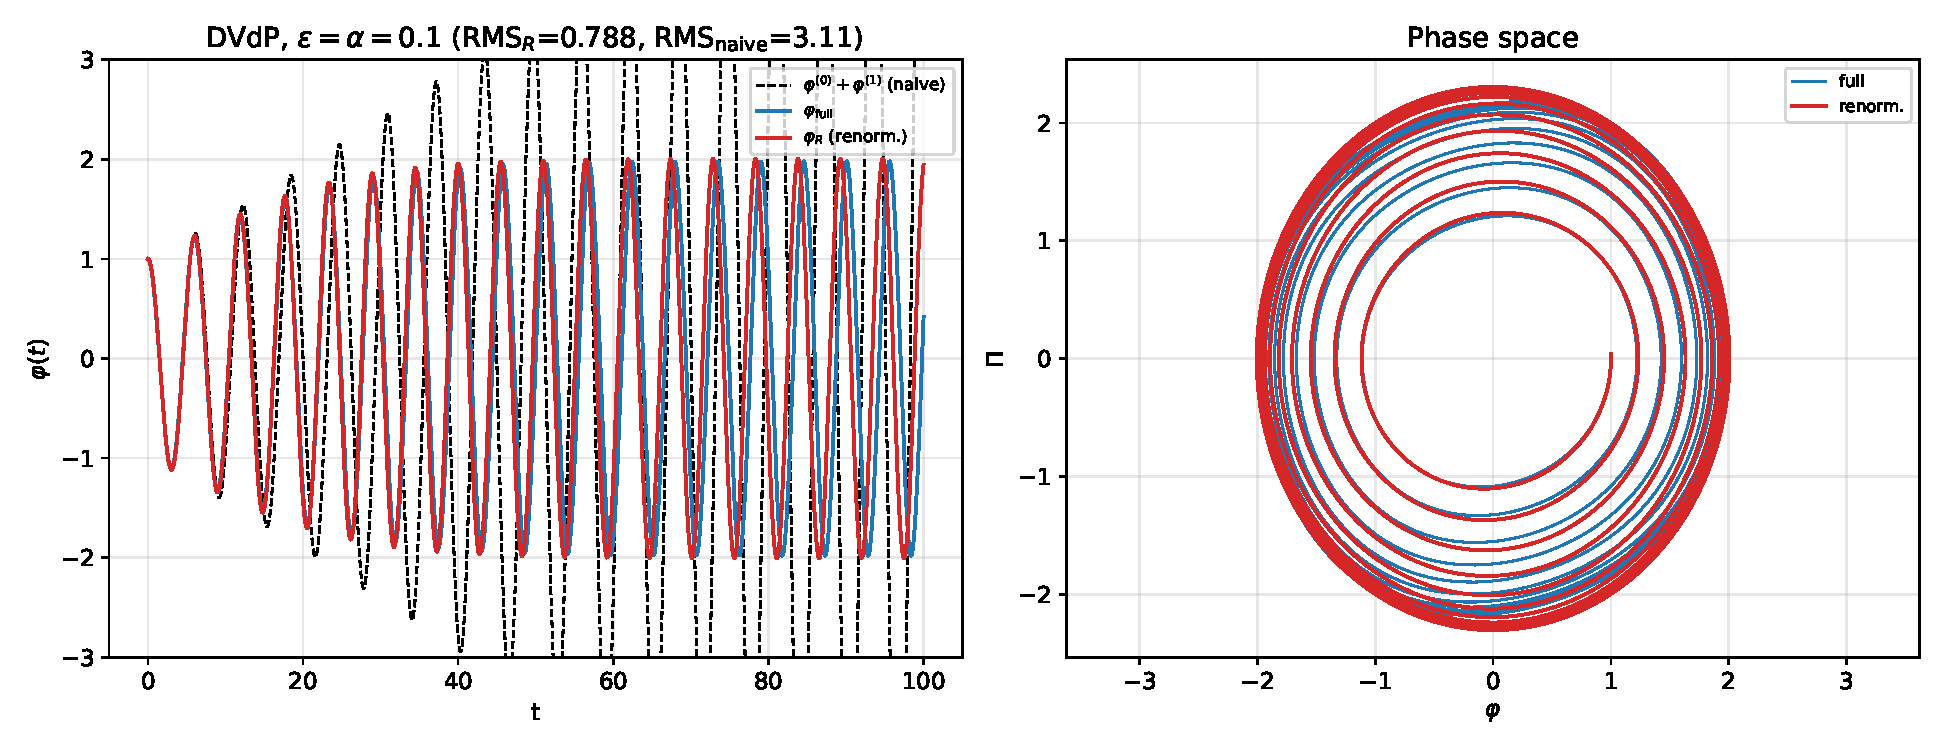
\includegraphics[width=\columnwidth]{fig_dvdp_soft.pdf}\\[2pt]
  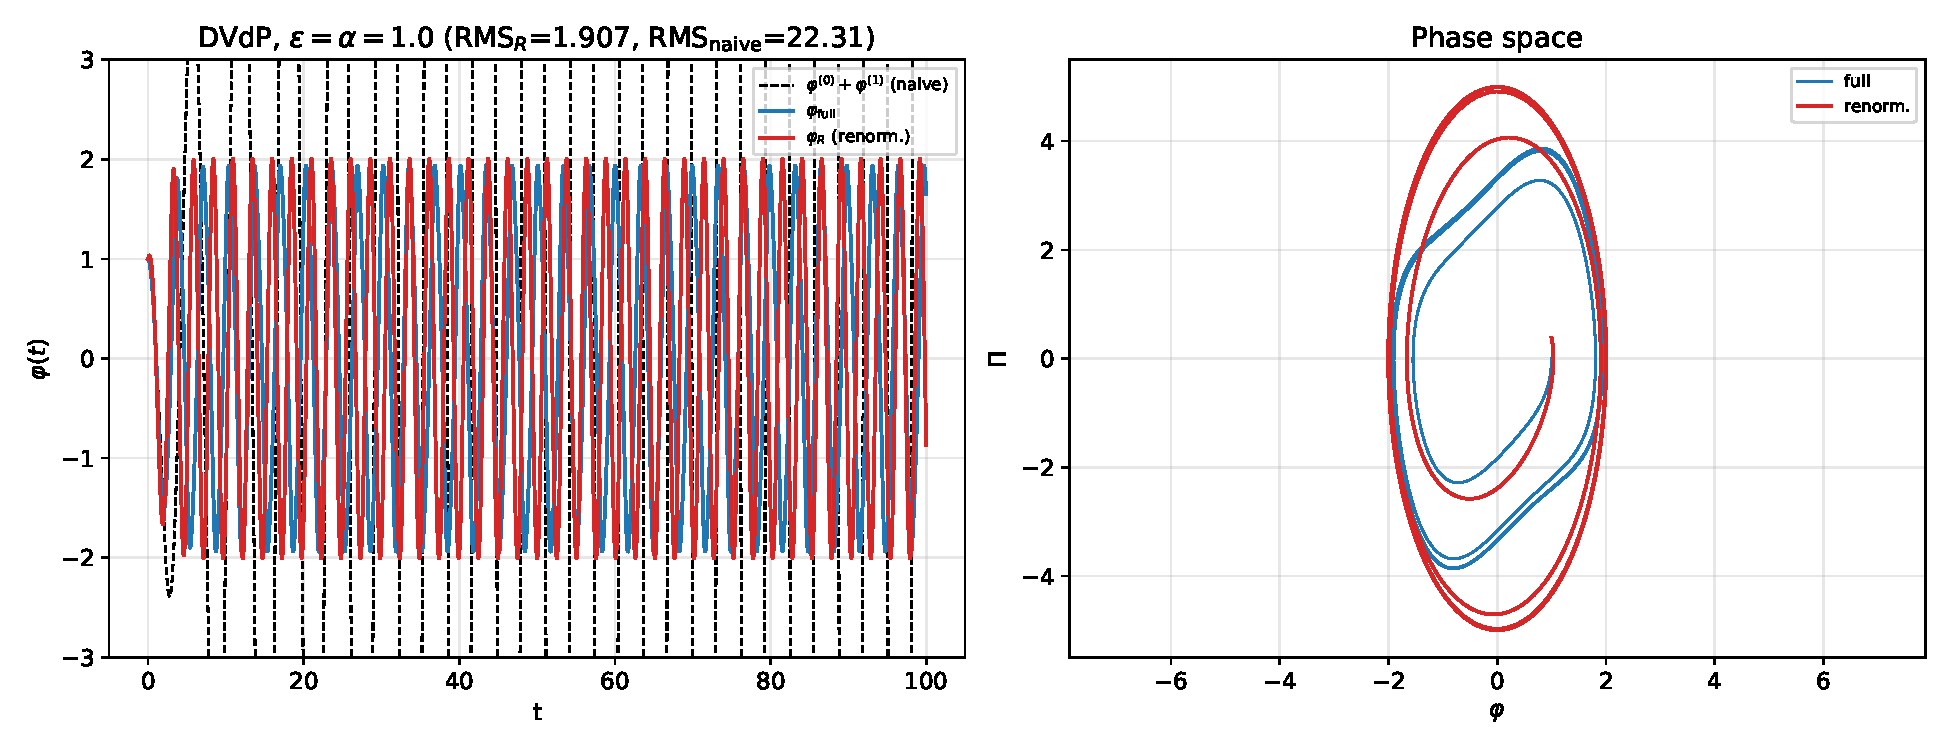
\includegraphics[width=\columnwidth]{fig_dvdp_strong.pdf}
  \caption{Combined DVdP oscillator. Top: soft coupling
  $\epsilon=\alpha=0.1$. Bottom: strong coupling $\epsilon=\alpha=1$. Left
  panels: time series (full, renormalized, naive). Right panels: phase-space
  portraits. The renormalized solution tracks the full one closely at soft
  coupling and captures the envelope and limit-cycle size at strong coupling.}
  \label{fig:dvdp}
\end{figure}

\section{Benchmarking}
\label{sec:benchmark}

\subsection{Choice of integrator}

The renormalization method only requires the first-order response, but a
reference (``full'') solution is needed to assess accuracy. We compared a
fixed-step fourth-order Runge--Kutta against the adaptive Runge--Kutta
(\texttt{RK45}), Dormand--Prince (\texttt{DOP853}) and implicit
(\texttt{Radau}) integrators of SciPy~\cite{virtanen2020} on the Duffing, Van
der Pol and combined systems. \texttt{DOP853} delivered the best accuracy per
right-hand-side evaluation on the non-stiff cases and reproduced the Van der
Pol limit cycle, while \texttt{Radau} was the most accurate but an order of
magnitude more expensive. We adopt \texttt{DOP853} (relative tolerance
$10^{-10}$) as the default reference integrator; the full table is provided in
the repository.

\subsection{Accuracy across coupling strengths}

Figure~\ref{fig:errscaling} reports the root-mean-square error of the
renormalized and naive solutions, relative to the full solution over
$t\in[0,100]$, as a function of the deformation strength. The renormalized
solution outperforms the naive perturbative one by roughly an order of
magnitude throughout, for all three systems, and remains bounded where the
naive solution diverges secularly.

\begin{figure}[t]
  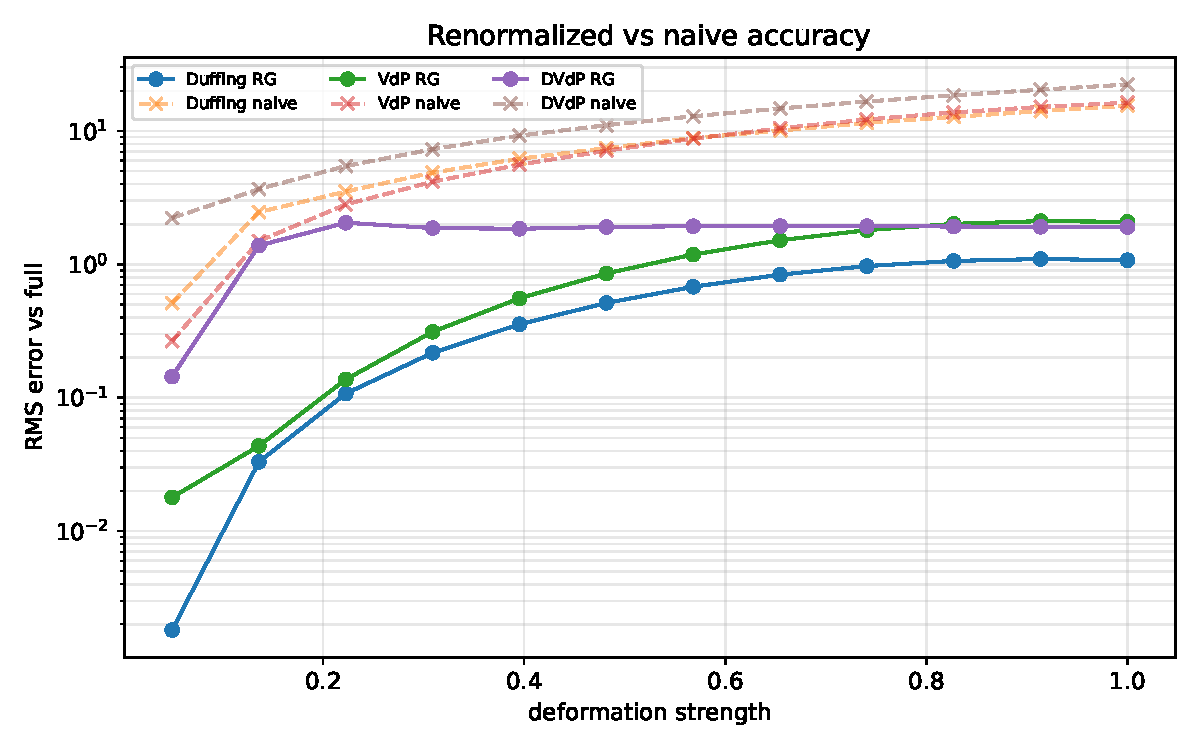
\includegraphics[width=\columnwidth]{fig_error_scaling.pdf}
  \caption{RMS error versus the full solution as a function of deformation
  strength, for Duffing, Van der Pol and the combined system. Solid: renormalized;
  dashed: naive first-order. The renormalized solution is consistently more
  accurate and avoids secular divergence.}
  \label{fig:errscaling}
\end{figure}

\section{Cases of study}
\label{sec:cases}

The combined DVdP oscillator is a minimal model of a self-sustained nonlinear
actuator with a stiffening restoring force, a setting common in nonlinear
control. Two benchmarking directions follow naturally from the method:

\begin{enumerate}
\item \emph{Semi-analytical surrogate.} Because the generators are extracted
once and stored as functions of amplitude, the renormalized flow
Eq.~\eqref{eq:flowDVdP} provides a fast, low-dimensional surrogate for the
oscillator's envelope and phase, suitable for real-time estimation where only
the linear (first-order) response of the plant is available.
\item \emph{Limit-cycle characterization.} The amplitude flow directly yields
the limit-cycle radius and its dependence on $(\epsilon,\alpha)$, which can be
compared against the Hopf-bifurcation analysis of related van der
Pol--Mathieu--Duffing models~\cite{roy2021}.
\end{enumerate}

A systematic comparison against multiple-scale and harmonic-balance
approximations, and an extension of the ansatz to include higher harmonics for
the strong-coupling limit cycle, are left for future work.

\section{Discussion}
\label{sec:discussion}

We have shown that a single numerical renormalization engine, built from the
first-order perturbative response, reproduces the Duffing frequency shift, the
Van der Pol amplitude flow, and---through the linear superposition of their
generators---the combined Duffing--Van der Pol dynamics for independent and
arbitrary deformation strengths, free of secular divergences. The method is
accurate from the weak-coupling regime up to moderately strong coupling; its
only essential limitation, a late-time phase drift at very strong coupling, is
inherited from the single-harmonic background ansatz and can be addressed by
enriching the parameter set. The construction requires only the linear response
of the system, making it attractive for nonlinear control applications where a
full analytic model is unavailable.

\begin{acknowledgments}
We thank the AFOSR program for support. Numerical work used
NumPy, SciPy and Matplotlib.
\end{acknowledgments}

\bibliographystyle{apsrev4-2}
\bibliography{refs}

\end{document}
